\documentclass[11pt,a4paper]{article}

% ─── Core Packages ───────────────────────────────────────────────────────────
\usepackage[margin=0.9in]{geometry}
\usepackage[T1]{fontenc}
\usepackage{lmodern}
\usepackage{amsmath,amssymb,amsthm}
\usepackage{mathtools}
\usepackage{graphicx}
\usepackage{xcolor}
\usepackage{booktabs}
\usepackage{multirow}
\usepackage{array}
\usepackage{enumitem}
\usepackage{algorithm}
\usepackage{algpseudocode}
\usepackage{tcolorbox}
\usepackage{microtype}
\usepackage{caption}
\usepackage{subcaption}
\usepackage{tikz}
\usepackage{pgfplots}
\pgfplotsset{compat=1.18}
\usetikzlibrary{positioning,arrows.meta,shapes.geometric,fit,calc,decorations.pathreplacing}
\usepackage{listings}
\usepackage{tabularx}
\usepackage{longtable}
\usepackage{float}
\usepackage{fancyhdr}
\usepackage{titlesec}
\usepackage{hyperref}
\usepackage[noabbrev]{cleveref}

% ─── Page Style ──────────────────────────────────────────────────────────────
\pagestyle{fancy}
\fancyhf{}
\fancyhead[L]{\small\textsc{TC-ViTok: Complete Project Specification}}
\fancyhead[R]{\small\thepage}
\renewcommand{\headrulewidth}{0.4pt}

% ─── Color Definitions ───────────────────────────────────────────────────────
\definecolor{defbg}{RGB}{245,240,255}
\definecolor{defborder}{RGB}{130,70,200}
\definecolor{warnbg}{RGB}{255,245,235}
\definecolor{warnborder}{RGB}{200,130,70}
\definecolor{notebg}{RGB}{235,245,255}
\definecolor{noteborder}{RGB}{70,130,200}
\definecolor{implbg}{RGB}{235,255,240}
\definecolor{implborder}{RGB}{70,180,100}
\definecolor{keybg}{RGB}{255,250,230}
\definecolor{keyborder}{RGB}{200,170,50}
\definecolor{codegray}{RGB}{248,248,248}
\definecolor{codekey}{RGB}{0,0,180}
\definecolor{codecomment}{RGB}{100,100,100}
\definecolor{codestring}{RGB}{160,32,32}
\definecolor{phasecolor}{RGB}{40,80,160}

% ─── Listings Setup ──────────────────────────────────────────────────────────
\lstset{
  language=Python,
  basicstyle=\ttfamily\footnotesize,
  keywordstyle=\color{codekey}\bfseries,
  commentstyle=\color{codecomment}\itshape,
  stringstyle=\color{codestring},
  backgroundcolor=\color{codegray},
  frame=single, framerule=0.4pt, rulecolor=\color{gray!40},
  numbers=left, numberstyle=\tiny\color{gray}, numbersep=6pt,
  breaklines=true, showstringspaces=false, tabsize=2,
  xleftmargin=12pt, xrightmargin=4pt,
  aboveskip=8pt, belowskip=8pt,
}

% ─── tcolorbox Environments ──────────────────────────────────────────────────
\tcbuselibrary{skins,breakable}

\newtcolorbox{definitionbox}[1][]{enhanced, breakable,
  colback=defbg, colframe=defborder, fonttitle=\bfseries\small,
  left=6pt, right=6pt, top=4pt, bottom=4pt, arc=4pt, #1}

\newtcolorbox{warnbox}[1][]{enhanced, breakable,
  colback=warnbg, colframe=warnborder, fonttitle=\bfseries\small,
  left=6pt, right=6pt, top=4pt, bottom=4pt, arc=4pt, #1}

\newtcolorbox{notebox}[1][]{enhanced, breakable,
  colback=notebg, colframe=noteborder, fonttitle=\bfseries\small,
  left=6pt, right=6pt, top=4pt, bottom=4pt, arc=4pt, #1}

\newtcolorbox{implbox}[1][]{enhanced, breakable,
  colback=implbg, colframe=implborder, fonttitle=\bfseries\small,
  left=6pt, right=6pt, top=4pt, bottom=4pt, arc=4pt, #1}

\newtcolorbox{keybox}[1][]{enhanced, breakable,
  colback=keybg, colframe=keyborder, fonttitle=\bfseries\small,
  left=6pt, right=6pt, top=4pt, bottom=4pt, arc=4pt, #1}

\newtcolorbox{phasebox}[1][]{enhanced, breakable,
  colback=phasecolor!5, colframe=phasecolor, fonttitle=\bfseries,
  left=6pt, right=6pt, top=6pt, bottom=6pt, arc=4pt, #1}

% ─── Math Operators ──────────────────────────────────────────────────────────
\DeclareMathOperator*{\argmin}{arg\,min}
\DeclareMathOperator*{\argmax}{arg\,max}
\DeclareMathOperator{\Softmax}{Softmax}
\DeclareMathOperator{\TopK}{Top\text{-}k}
\DeclareMathOperator{\Concat}{Concat}
\DeclareMathOperator{\Upsample}{Upsample}
\DeclareMathOperator{\reshape}{reshape}
\DeclareMathOperator{\flatten}{flatten}
\DeclareMathOperator{\IoU}{IoU}
\DeclareMathOperator{\simop}{sim}
\DeclareMathOperator{\GELU}{GELU}
\newcommand{\sg}[1]{\mathrm{sg}\!\left[#1\right]}

% ─── Math Shorthands ─────────────────────────────────────────────────────────
\newcommand{\R}{\mathbb{R}}
\newcommand{\E}{\mathbb{E}}
\newcommand{\vc}{\mathbf{v}_c}
\newcommand{\qe}{\mathbf{q}_e}
\newcommand{\vm}{\mathbf{m}}
\newcommand{\vs}{\mathbf{s}}
\newcommand{\mI}{\mathbf{I}}
\newcommand{\mQ}{\mathbf{Q}}
\newcommand{\mV}{\mathbf{V}}

% ─── Theorem Environments ────────────────────────────────────────────────────
\newtheorem{hypothesis}{Hypothesis}
\newtheorem{remark}{Remark}
\newtheorem{definition}{Definition}
\newtheorem{proposition}{Proposition}

% ─── Section Formatting ──────────────────────────────────────────────────────
\titleformat{\section}{\Large\bfseries\color{phasecolor}}{\thesection}{1em}{}
\titleformat{\subsection}{\large\bfseries}{\thesubsection}{0.8em}{}

% ─── Hyperref Setup ──────────────────────────────────────────────────────────
\hypersetup{
  colorlinks=true, linkcolor=defborder, citecolor=teal, urlcolor=noteborder,
  pdftitle={TC-ViTok: Complete Project Specification},
  pdfauthor={Muhammad Ali Shah and Talha Hassan Ul Haq}
}

% ════════════════════════════════════════════════════════════════════════════
\begin{document}
% ════════════════════════════════════════════════════════════════════════════

\title{
  \textbf{TC-ViTok: Task-Conditioned Visual Tokenizer} \\[0.4em]
  \Large Complete Project Specification \\[0.3em]
  \large From Theory to Fully Buildable, Experimentally Validated System
}

\author{
  Muhammad Ali Shah - Talha Hassan Ul Haq \\[0.3em]
  Lahore University of Management Sciences (LUMS) \\
  \texttt{\{27100172, 27100306\}@lums.edu.pk}
}

\date{\today}
\maketitle
\thispagestyle{empty}

\begin{abstract}
This document provides a complete, end-to-end project specification for
\textbf{TC-ViTok} (Task-Conditioned Visual Tokenizer), a system that learns
to select visual tokens conditioned on the user's language query in
vision-language models. Selected tokens are extracted via
\textbf{index-gather} before LLM injection, reducing the LLM prefill
sequence from $N{+}L$ to $k{+}L$ tokens and cutting prefill FLOPs by up
to $75\%$ at $k{=}144$. The specification spans deep theoretical
foundations, full mathematical derivations with tensor shapes at every step,
complete architecture design, step-by-step PyTorch implementation,
experimental validation strategy, failure mode catalog, and a week-by-week
execution roadmap.
\end{abstract}

\tableofcontents
\newpage

% ════════════════════════════════════════════════════════════════════════════
\section{Core Idea and System Overview}
\label{sec:overview}
% ════════════════════════════════════════════════════════════════════════════

\subsection{Problem Statement}

\begin{definitionbox}[title={The Fixed-Budget Problem}]
Vision-Language Models such as LLaVA-1.5 encode every input image into a
\textbf{fixed-length sequence} of $N = 576$ visual tokens (from a
$336 \times 336$ image with $14 \times 14$ patches). These tokens are
concatenated with $L$ text tokens and processed by a causal LLM:
\begin{equation}
  \text{Cost}_{\text{prefill}} = \mathcal{O}\bigl(N(N + L) + L^2\bigr).
\end{equation}
For $N = 576$ and $L \approx 30$, visual tokens account for $\sim\!95\%$
of prefill cost. \textbf{The core problem}: the visual token budget is
determined by image resolution, not by the task.
\end{definitionbox}

\subsection{Why Current Methods Fail}

\begin{table}[h]
\centering
\caption{Limitations of existing visual token compression methods.}
\label{tab:existing_methods}
\renewcommand{\arraystretch}{1.2}
\small
\begin{tabular}{@{}lccll@{}}
  \toprule
  Method & Query-Aware & Where Saved & Core Limitation \\
  \midrule
  ToMe & No & ViT + LLM & Merges by visual similarity only \\
  LLaVA-PruMerge & No & LLM only & Uses {[CLS]} (whole-image summary) \\
  DynamicViT & No & ViT + LLM & Content-adaptive, task-agnostic \\
  BLIP-2 Q-Former & Partially & Both & Learned queries, not user query \\
  \bottomrule
\end{tabular}
\end{table}

\noindent All existing methods share one limitation: \textbf{the compression
decision is made without knowledge of what the user is asking}.
Several also apply zero-masking (retaining sequence length $N$), which
saves KV-cache memory but not prefill FLOPs.

\subsection{What TC-ViTok Does}

TC-ViTok introduces a \textbf{Tokenization Policy Network (TPN)}---a
lightweight cross-attention module that:
\begin{enumerate}[leftmargin=1.5em, itemsep=2pt]
  \item Takes the user's language query
    ($\to \qe \in \R^{512}$ via frozen CLIP text encoder).
  \item Takes a coarse spatial map of the image
    ($\to \vc \in \R^{49 \times 384}$ via frozen DINOv2-S).
  \item Produces a ranked score vector $\vs_N \in \R^{576}$ and selects
    the top-$k$ token indices $\mathcal{S}$.
  \item \textbf{Gathers} the selected rows from the full ViT-L output:
    $\mV_\mathcal{S} = \mV[\mathcal{S},:] \in \R^{k \times d_v}$.
  \item Passes $\mV_\mathcal{S}$ to the LLM, which now sees a sequence
    of length $k{+}L$ instead of $N{+}L$.
\end{enumerate}

\textbf{The novelty}: the token selection decision is conditioned on the
user's specific natural-language query, \emph{and} realized via gather
so that the LLM prefill sequence is genuinely shortened.

\subsection{System Architecture}

\begin{figure}[t]
\centering
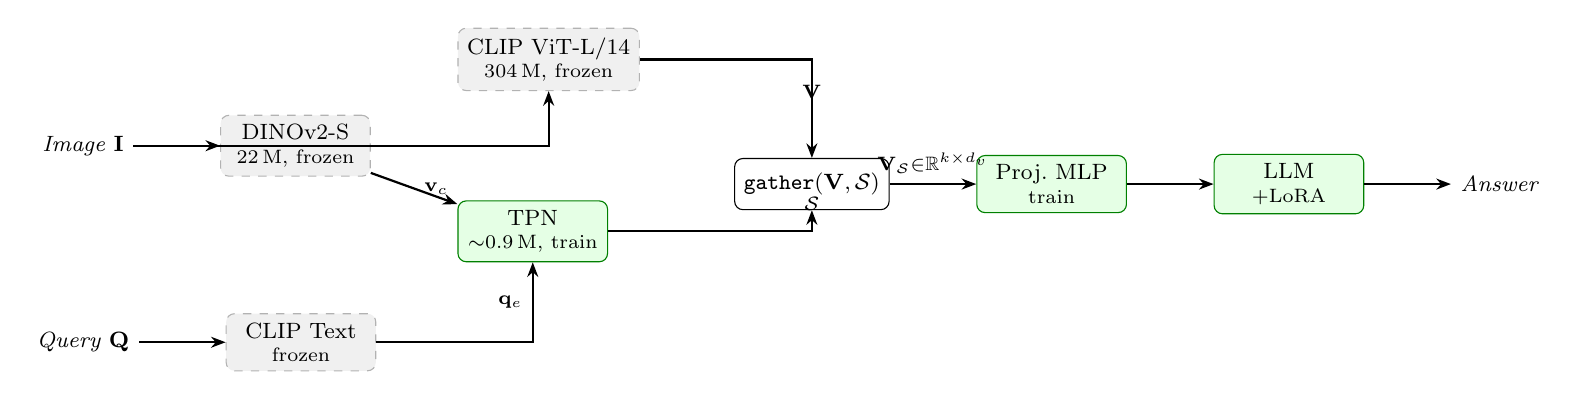
\begin{tikzpicture}[
    node distance=0.55cm and 1.1cm,
    block/.style={rectangle, draw, rounded corners=3pt,
                  minimum height=0.65cm, minimum width=1.9cm,
                  font=\footnotesize, align=center, fill=white},
    frozen/.style={block, fill=gray!12, draw=gray!60, dashed},
    trainable/.style={block, fill=green!10, draw=green!50!black},
    data/.style={font=\footnotesize\itshape, align=center},
    arr/.style={-{Stealth[scale=0.8]}, thick},
    label/.style={font=\scriptsize},
]
  \node[data] (img) {Image $\mI$};
  \node[data, below=2.0cm of img] (query) {Query $\mQ$};
  \node[frozen, right=of img] (dino)
    {DINOv2-S\\[-1pt]{\scriptsize 22\,M, frozen}};
  \node[frozen, right=of query] (clip)
    {CLIP Text\\[-1pt]{\scriptsize frozen}};
  \node[frozen, above right=0.3cm and 1.1cm of dino] (vit)
    {CLIP ViT-L/14\\[-1pt]{\scriptsize 304\,M, frozen}};
  \node[trainable, below right=0.3cm and 1.1cm of dino] (tpn)
    {TPN\\[-1pt]{\scriptsize $\sim$0.9\,M, train}};
  \node[block, right=1.6cm of tpn, yshift=0.6cm] (gather)
    {\texttt{gather}$(\mV,\mathcal{S})$};
  \node[trainable, right=of gather] (mlp)
    {Proj.\ MLP\\[-1pt]{\scriptsize train}};
  \node[trainable, right=of mlp] (llm)
    {LLM\\[-1pt]{\scriptsize +LoRA}};
  \node[data, right=of llm] (ans) {Answer};
  \draw[arr] (img) -- (dino);
  \draw[arr] (img) -| (vit);
  \draw[arr] (query) -- (clip);
  \draw[arr] (dino) -- (tpn) node[midway,right,label]{$\vc$};
  \draw[arr] (clip) -| (tpn) node[near end,left,label]{$\qe$};
  \draw[arr] (tpn) -| (gather) node[near end,above,label]{$\mathcal{S}$};
  \draw[arr] (vit) -| (gather) node[near end,above,label]{$\mV$};
  \draw[arr] (gather) -- (mlp)
    node[midway,above,label]{$\mV_\mathcal{S}{\in}\R^{k\times d_v}$};
  \draw[arr] (mlp) -- (llm);
  \draw[arr] (llm) -- (ans);
\end{tikzpicture}
\caption{TC-ViTok system architecture. Gray dashed: frozen components.
Green: trainable (TPN, projection MLP, LoRA adapters). The TPN produces
a token index set $\mathcal{S}$ conditioned on $\qe$ and $\vc$.
A \texttt{gather} operation extracts $\mV_\mathcal{S} \in \R^{k \times d_v}$,
the compact visual sequence that enters the LLM (length $k{+}L$, not $N{+}L$).}
\label{fig:architecture}
\end{figure}

\subsection{End-to-End Data Flow with Shapes}

\begin{table}[h]
\centering
\caption{Complete data flow through TC-ViTok with tensor shapes (batch $B$).}
\label{tab:data_flow}
\renewcommand{\arraystretch}{1.15}
\small
\begin{tabular}{@{}clllc@{}}
  \toprule
  Step & Operation & Input Shape & Output Shape & Frozen? \\
  \midrule
  1  & Resize for coarse        & $(B,3,336,336)$     & $(B,3,98,98)$       & --- \\
  2  & DINOv2-S forward         & $(B,3,98,98)$       & $(B,49,384)$        & Yes \\
  3  & CLIP text encode         & Token IDs $(B,L)$   & $(B,512)$           & Yes \\
  4  & CLIP ViT-L/14            & $(B,3,336,336)$     & $(B,576,1024)$      & Yes \\
  5  & TPN: Q projection        & $(B,512)$           & $(B,1,384)$         & No  \\
  6  & TPN: K/V projection      & $(B,49,384)$        & $(B,49,384)\times2$ & No  \\
  7  & TPN: cross-attn          & Q,K,V               & ctx$(B,384)$, $\alpha(B,49)$ & No \\
  8  & TPN: score MLP           & $(B,433)$           & $(B,49)$            & No  \\
  9  & TPN: upsample            & $(B,1,7,7)$         & $(B,576)$           & No  \\
  10 & Top-$k$ index selection  & $(B,576)$           & \textbf{idx} $(B,144)$   & No  \\
  11 & \textbf{Gather} (Option B) & $(B,576,1024)$ + $(B,144)$ & \boldmath$(B,144,1024)$ & --- \\
  12 & Projection MLP           & $(B,144,1024)$      & $(B,144,4096)$      & No  \\
  13 & Concat with text         & Visual + Text       & $(B,\mathbf{144}{+}L,4096)$ & --- \\
  14 & LLM forward (+LoRA)      & $(B,144{+}L,4096)$  & $(B,144{+}L,|\mathcal{V}|)$ & Partial \\
  \bottomrule
\end{tabular}
\end{table}

\begin{notebox}[title={Why gather, not zero-masking}]
Zero-masking (multiplying $\mV$ by a binary mask and retaining all 576 rows)
keeps the LLM sequence at length $N{+}L$, saving KV-cache memory but
\emph{not} prefill FLOPs. Gather reduces the sequence to $k{+}L$, saving
both. Since $k$ is fixed ($=144$) for all batch items, no variable-length
padding is needed---gather produces a uniformly shaped $(B, k, d_v)$ tensor.
\end{notebox}

\subsection{Component Summary}

\begin{table}[h]
\centering
\caption{System components: parameters and trainability.}
\label{tab:components}
\renewcommand{\arraystretch}{1.15}
\small
\begin{tabular}{@{}lrcc@{}}
  \toprule
  Component & Parameters & Trainable & Role \\
  \midrule
  DINOv2-Small      & 22\,M        & No      & Cheap spatial features for TPN \\
  CLIP Text Encoder & $\sim$63\,M  & No      & Query embedding \\
  CLIP ViT-L/14     & 304\,M       & No      & Full visual tokens \\
  \textbf{TPN}      & \textbf{$\sim$0.9\,M} & \textbf{Yes} & \textbf{Query-conditioned spatial scoring} \\
  Projection MLP    & $\sim$8\,M   & Yes     & Map visual $\to$ LLM space \\
  Vicuna-7B (LoRA)  & 7\,B ($\sim$25\,M LoRA) & Partial & Answer generation \\
  \bottomrule
\end{tabular}
\end{table}

% ════════════════════════════════════════════════════════════════════════════
\section{Full Mathematical Foundation}
\label{sec:math}
% ════════════════════════════════════════════════════════════════════════════

\subsection{Complete Notation}

\begin{table}[t]
\centering
\caption{Complete notation reference.}
\label{tab:notation}
\renewcommand{\arraystretch}{1.2}
\small
\begin{tabular}{@{}llp{7cm}@{}}
  \toprule
  Symbol & Shape & Description \\
  \midrule
  \multicolumn{3}{@{}l}{\emph{Inputs}} \\
  $\mI$ & $H{\times}W{\times}3$ & Raw input image \\
  $\mI_c$ & $98{\times}98{\times}3$ & Image resized for coarse encoder \\
  $\mQ = (q_1,\ldots,q_L)$ & sequence & Language query tokens \\[3pt]
  \multicolumn{3}{@{}l}{\emph{Intermediate representations}} \\
  $\vc \in \R^{M \times d_c}$ & $49{\times}384$ & Coarse DINOv2-S spatial features \\
  $\qe \in \R^{d_q}$ & $512$ & CLIP text [EOS] embedding \\
  $\mV \in \R^{N \times d_v}$ & $576{\times}1024$ & Full CLIP ViT-L/14 visual embeddings \\[3pt]
  \multicolumn{3}{@{}l}{\emph{TPN outputs}} \\
  $\vs_M \in \R^{M}$ & $49$ & Coarse spatial relevance scores \\
  $\vs_N \in \R^{N}$ & $576$ & Full-resolution scores (upsampled) \\
  $\mathcal{S} \subseteq \{1,\ldots,N\}$ & $|\mathcal{S}|{=}k$ & Selected token \textbf{index set} \\
  $\mV_{\mathcal{S}} \in \R^{k \times d_v}$ & $\mathbf{144{\times}1024}$
    & \textbf{Gathered} visual tokens (compact, $k$ rows only) \\[3pt]
  \multicolumn{3}{@{}l}{\emph{Hyperparameters}} \\
  $N = (H/p)^2$ & $576$ & Total visual tokens ($p{=}14$, $H{=}336$) \\
  $k$ & $144$ (default) & Token budget \\
  $\tau$ & scalar & Gumbel-Sigmoid temperature \\
  $\lambda, \mu, \nu$ & scalars & Loss coefficients \\
  \bottomrule
\end{tabular}
\end{table}

\subsection{The Optimization Objective}

\begin{definitionbox}[title={TC-ViTok Training Objective}]
\begin{equation}
  \theta^* = \argmin_{\theta} \;
    \E_{(\mI,\mQ,A)\sim\mathcal{D}} \Big[
      \underbrace{
        -\log P\!\left(A \mid \mQ,\,\mV_{\mathcal{S}_\theta}\right)
      }_{\mathcal{L}_{\text{VQA}}}
      \;+\; \underbrace{
        \lambda \cdot \frac{\lVert \vs_\theta \rVert_1}{N}
      }_{\mathcal{L}_{\text{comp}}}
      \;+\; \underbrace{
        \mu \cdot \mathcal{L}_{\text{ent}}
      }_{\text{diversity}}
    \Big]
  \label{eq:objective}
\end{equation}
where $\mathcal{S}_\theta = \TopK(\vs_\theta(\qe,\vc),\, k)$,
$\mV_{\mathcal{S}_\theta} = \mV[\mathcal{S}_\theta, :] \in \R^{k \times d_v}$
is the \textbf{gathered} visual sequence, and $A$ is the ground-truth answer.
\end{definitionbox}

\subsection{Cross-Attention Derivation (Step-by-Step)}
\label{subsec:cross_attn_deriv}

\subsubsection{Input Setup}

\begin{itemize}[leftmargin=1.5em, itemsep=1pt]
  \item Query embedding: $\qe \in \R^{d_q}$, $d_q = 512$
  \item Coarse visual tokens: $\vc \in \R^{M \times d_c}$, $M = 49$, $d_c = 384$
  \item Model dimension: $d_{\text{model}} = 384$; Heads: $H = 4$; $d_k = 96$
\end{itemize}

\subsubsection{Step 1--6: Cross-Attention}

\begin{equation}
  \mathbf{Q} = \qe\,\mathbf{W}^Q \in \R^{1 \times 384}, \quad
  \mathbf{K} = \vc\,\mathbf{W}^K \in \R^{49 \times 384}, \quad
  \mathbf{V} = \vc\,\mathbf{W}^V \in \R^{49 \times 384}
\end{equation}

After multi-head reshape (batch $B$):
$\mathbf{Q}\!:(B,4,1,96)$, $\mathbf{K}\!:(B,4,49,96)$, $\mathbf{V}\!:(B,4,49,96)$.

\begin{equation}
  \boldsymbol{\alpha}^{(h)} = \Softmax\!\!\left(
    \frac{\mathbf{Q}^{(h)}{\mathbf{K}^{(h)}}^\top}{\sqrt{96}}
  \right) \in \R^{B \times 1 \times 49}
\end{equation}

\begin{equation}
  \bar{\boldsymbol{\alpha}} = \frac{1}{H}\sum_h \boldsymbol{\alpha}^{(h)}
  \in \R^{B \times 49}, \qquad
  \mathbf{a} = \Concat(\mathbf{a}^{(1)},\ldots)\,\mathbf{W}^O
  \in \R^{B \times 384}
\end{equation}

\subsection{Spatial Scoring and Upsampling}

\begin{equation}
  \mathbf{h} = \GELU(\mathbf{W}_1[\mathbf{a};\bar{\boldsymbol{\alpha}}] + \mathbf{b}_1)
  \in \R^{B \times 512}, \qquad
  \vs_M = \mathbf{W}_2\mathbf{h} + \mathbf{b}_2 \in \R^{B \times 49}
\end{equation}

\begin{equation}
  \vs_N = \flatten\!\bigl(\Upsample(\reshape(\vs_M, 7,7),\,(24,24))\bigr)
  \in \R^{B \times 576}
\end{equation}

\subsection{Gather-Based Token Extraction}

From $\vs_N$, select top-$k$ indices and gather:
\begin{equation}
  \mathcal{S} = \TopK(\vs_N, k), \qquad
  \mV_\mathcal{S} = \mV[\mathcal{S}, :]
  = \texttt{torch.gather}(\mV,\, \text{dim}{=}1,\, \mathcal{S}^{\uparrow d_v})
  \in \R^{B \times k \times d_v}
  \label{eq:gather}
\end{equation}
where $\mathcal{S}^{\uparrow d_v}$ denotes expanding the index tensor to
$(B, k, d_v)$.
This is the \textbf{only} masking operation; no zero-padding or sequence
truncation is applied. The LLM receives a sequence of length $k{+}L$.

\subsection{Gumbel-Sigmoid STE}

\begin{definitionbox}[title={Gumbel-Sigmoid Soft Mask}]
\begin{equation}
  \tilde{m}_i(\tau)
    = \sigma\!\left(\frac{s_{N,i} + g_i}{\tau}\right), \quad
  g_i = -\log(-\log(u_i)), \quad u_i \sim \text{Uniform}(0,1)
  \label{eq:gumbel_sigmoid}
\end{equation}
\end{definitionbox}

\begin{definitionbox}[title={Straight-Through Estimator for Top-$k$}]
\begin{align}
  \vm_{\text{hard}} &= \mathbf{1}[\vs_N \geq \tau_k(\vs_N)]
    && \text{(forward pass)} \\
  \tilde{\vm}(\tau) &= \sigma((\vs_N + \mathbf{g})/\tau)
    && \text{(backward-pass gradients)} \\
  \vm_{\text{STE}} &= \vm_{\text{hard}} - \sg{\tilde{\vm}(\tau)} + \tilde{\vm}(\tau)
    \label{eq:ste}
\end{align}
At training time, gather indices are derived from $\vm_{\text{hard}}$
(positions where $\vm_{\text{STE}} = 1$), so gradients flow through
$\tilde{\vm}$ to TPN parameters.
\end{definitionbox}

\subsection{Temperature Annealing and Loss Schedules}

\begin{equation}
  \tau(t) = \tau_{\max} - (\tau_{\max} - \tau_{\min}) \cdot \frac{t}{T},
  \quad \tau_{\max}{=}1.0,\; \tau_{\min}{=}0.1
\end{equation}

\begin{equation}
  \lambda(t) = \lambda_{\max} \cdot \min\!\left(1,\;\frac{t}{T_{\text{warmup}}}\right)
\end{equation}

\begin{definitionbox}[title={Full Training Loss}]
\begin{equation}
  \mathcal{L}(t) =
    \underbrace{-\log P(A \mid \mQ, \mV_\mathcal{S})}_{\text{VQA}}
    + \underbrace{\lambda(t) \cdot \frac{\|\vs_N\|_1}{N}}_{\text{sparsity}}
    - \underbrace{|\mu| \cdot \mathcal{L}_{\text{ent}}}_{\text{diversity}}
    + \underbrace{\nu \cdot \mathcal{L}_{\text{div}}}_{\text{query diversity}}
  \label{eq:total_loss}
\end{equation}
Defaults: $\lambda_{\max}{=}0.1$, $|\mu|{=}0.01$, $\nu{=}0.01$.
\end{definitionbox}

% ════════════════════════════════════════════════════════════════════════════
\section{Architecture Deep Dive}
\label{sec:architecture}
% ════════════════════════════════════════════════════════════════════════════

\subsection{Component 1: Coarse Visual Encoder (DINOv2-Small)}

\begin{itemize}[leftmargin=1.5em, itemsep=1pt]
  \item Architecture: ViT-Small (12 layers, 6 heads, 384 hidden dim)
  \item Patch size: 14, input: $98{\times}98 \Rightarrow 7{\times}7 = 49$ tokens
  \item Output: $(B, 49, 384)$ (CLS excluded). Parameters: 22\,M (frozen)
\end{itemize}

\begin{warnbox}[title={Critical Normalization Warning}]
DINOv2: \texttt{mean=[0.485, 0.456, 0.406]}, \texttt{std=[0.229, 0.224, 0.225]}.
CLIP:    \texttt{mean=[0.481, 0.458, 0.408]}, \texttt{std=[0.269, 0.261, 0.276]}.
Applying CLIP normalization to DINOv2 is a \textbf{silent, hard-to-debug error}.
\end{warnbox}

\subsection{Component 2: Text Encoder (CLIP ViT-B/32)}

Output: $\qe \in \R^{B \times 512}$ ([EOS] token embedding, frozen).
Mean-pooling is not used: CLIP training concentrates global semantics in [EOS].

\subsection{Component 3: Tokenization Policy Network (TPN)}

Maps $(\qe, \vc) \mapsto \vs_N \in \R^N$ and selected indices $\mathcal{S}$.
Internal pipeline: Q/K/V projections $\to$ multi-head cross-attention
$\to$ score MLP $\to$ bilinear upsample $\to$ top-$k$ index selection.

\begin{table}[h]
\centering
\caption{TPN parameter count.}
\label{tab:tpn_params}
\renewcommand{\arraystretch}{1.15}
\small
\begin{tabular}{@{}lr@{}}
  \toprule
  Component & Parameters \\
  \midrule
  $\mathbf{W}^Q$ ($512 \times 384$)      & 196{,}608 \\
  $\mathbf{W}^K$ ($384 \times 384$)      & 147{,}456 \\
  $\mathbf{W}^V$ ($384 \times 384$)      & 147{,}456 \\
  $\mathbf{W}^O$ ($384 \times 384$)      & 147{,}456 \\
  LayerNorm $\times 2$                   & 1{,}634   \\
  Score MLP $\mathbf{W}_1$ ($433\times512$+bias) & 222{,}208 \\
  Score MLP $\mathbf{W}_2$ ($512\times49$+bias)  & 25{,}137  \\
  \midrule
  \textbf{Total} & \textbf{887{,}955 ($\approx$0.9\,M)} \\
  \bottomrule
\end{tabular}
\end{table}

\subsection{Component 4: Gather-Based Token Extraction}
\label{subsec:gather_component}

Given $\vs_N \in \R^{B \times N}$ from the TPN and
$\mV \in \R^{B \times N \times d_v}$ from the frozen ViT-L:

\begin{equation}
  \text{idx} = \vs_N.\texttt{topk}(k, \text{dim}{=}{-}1).\texttt{indices}
  \quad\in \R^{B \times k}
\end{equation}

\begin{equation}
  \mV_\mathcal{S} = \texttt{torch.gather}(\mV,\; \text{dim}{=}1,\;
  \text{idx.unsqueeze}({-}1)\texttt{.expand}({-}1,{-}1,d_v))
  \quad\in \R^{B \times k \times d_v}
\end{equation}

This is the \textbf{only} masking operation. The resulting compact tensor
$\mV_\mathcal{S} \in \R^{B \times 144 \times 1024}$ goes directly to the
projection MLP. The LLM receives a combined sequence of length $144{+}L$,
not $576{+}L$.

\paragraph{Why gather, not zero-masking.}
Zero-masking retains shape $(B, 576, d_v)$; the LLM still computes
attention over all 576 positions, saving only KV-cache memory.
Gather produces shape $(B, 144, d_v)$; LLM attention cost scales as
$\mathcal{O}(k^2)$ instead of $\mathcal{O}(N^2)$, giving genuine FLOP
reduction. Since $k$ is fixed across the batch, no variable-length
handling is required.

\paragraph{Computational overhead.}
\begin{itemize}[leftmargin=1.5em, itemsep=1pt]
  \item DINOv2-S forward: $\sim$3\,ms; CLIP text: $\sim$2\,ms; TPN: $\sim$0.5\,ms
  \item Total overhead: $\sim$5.5\,ms
  \item LLM savings via gather ($k{=}144$): $\sim$40\,ms
  \item \textbf{Net savings: $\sim$34\,ms} per sample at batch size 1 on A100
\end{itemize}

% ════════════════════════════════════════════════════════════════════════════
\section{Full Implementation Guide}
\label{sec:implementation}
% ════════════════════════════════════════════════════════════════════════════

\subsection{Stage A: Environment Setup}

\begin{implbox}[title={Required Libraries}]
\begin{lstlisting}[numbers=none, language=bash]
pip install torch==2.1.0 torchvision==0.16.0
pip install transformers==4.36.2 accelerate==0.25.0 peft==0.7.1
pip install timm==0.9.12
pip install datasets==2.16.0 h5py==3.10.0 Pillow==10.1.0
pip install wandb tqdm
\end{lstlisting}
\end{implbox}

\begin{table}[h]
\centering
\caption{Required model checkpoints.}
\renewcommand{\arraystretch}{1.15}
\small
\begin{tabular}{@{}llr@{}}
  \toprule
  Model & HuggingFace ID & Size \\
  \midrule
  LLaVA-1.5-7B & \texttt{llava-hf/llava-1.5-7b-hf} & $\sim$13.5\,GB \\
  DINOv2-Small  & \texttt{facebook/dinov2-small}       & $\sim$88\,MB   \\
  CLIP ViT-B/32 & \texttt{openai/clip-vit-base-patch32} & $\sim$340\,MB \\
  \bottomrule
\end{tabular}
\end{table}

\subsection{Stage B: Data Pipeline}

\begin{lstlisting}[caption={Separate preprocessing for DINOv2 and CLIP.}]
from torchvision import transforms

# DINOv2 preprocessing (ImageNet normalization)
dino_transform = transforms.Compose([
    transforms.Resize((98, 98)),
    transforms.ToTensor(),
    transforms.Normalize(
        mean=[0.485, 0.456, 0.406],
        std=[0.229, 0.224, 0.225]
    )
])
# CLIP ViT-L preprocessing handled by LLaVA processor:
# Resize 336x336; mean=[0.481,0.458,0.408]; std=[0.269,0.261,0.276]
\end{lstlisting}

\begin{lstlisting}[caption={Pre-compute and cache frozen encoder outputs.}]
import h5py, torch
from tqdm import tqdm

def precompute_features(dataset, output_path, device='cuda'):
    dino = torch.hub.load('facebookresearch/dinov2','dinov2_vits14')
    dino = dino.to(device).eval()
    clip_model = CLIPModel.from_pretrained("openai/clip-vit-base-patch32")
    clip_text = clip_model.text_model.to(device).eval()
    tokenizer = CLIPTokenizer.from_pretrained("openai/clip-vit-base-patch32")

    n = len(dataset)
    with h5py.File(output_path, 'w') as f:
        f.create_dataset('dino_features', shape=(n, 49, 384), dtype='float16')
        f.create_dataset('clip_text_emb', shape=(n, 512),    dtype='float16')
        for i in tqdm(range(n)):
            sample = dataset[i]
            img = dino_transform(sample['image']).unsqueeze(0).to(device)
            with torch.no_grad():
                out = dino.forward_features(img)
                v_c = out['x_norm_patchtokens']       # (1, 49, 384)
                f['dino_features'][i] = v_c.cpu().half().numpy()
            tokens = tokenizer(sample['question'], return_tensors='pt',
                               padding='max_length', max_length=77,
                               truncation=True).to(device)
            with torch.no_grad():
                text_out = clip_text(**tokens)
                eos_idx = tokens['attention_mask'].sum(1) - 1
                q_e = text_out.last_hidden_state[0, eos_idx[0]]
                f['clip_text_emb'][i] = q_e.cpu().half().numpy()
\end{lstlisting}

\subsection{Stage C: Model Implementation}

\subsubsection{Gumbel-Sigmoid STE}

\begin{lstlisting}[caption={Gumbel-Sigmoid STE (returns soft mask for grad flow).}]
import torch

def gumbel_sigmoid_ste(scores, k, tau):
    """
    Args:
        scores: (B, N) raw spatial scores from TPN
        k:      number of tokens to select
        tau:    temperature (annealed 1.0 -> 0.1)
    Returns:
        mask_ste: (B, N) binary in fwd, soft grads in bwd
        idx:      (B, k) top-k indices for gather
    """
    eps = 1e-8
    u = torch.rand_like(scores).clamp(eps, 1 - eps)
    g = -torch.log(-torch.log(u))                    # Gumbel(0,1)
    m_soft = torch.sigmoid((scores + g) / tau)        # (B, N)

    idx = scores.topk(k, dim=-1).indices              # (B, k)
    m_hard = torch.zeros_like(scores)
    m_hard.scatter_(-1, idx, 1.0)

    mask_ste = m_hard - m_soft.detach() + m_soft      # STE
    return mask_ste, idx
\end{lstlisting}

\subsubsection{Gather Helper}

\begin{lstlisting}[caption={Gather top-k visual tokens (Option B).}]
def gather_tokens(V, idx):
    """
    Extract k visual tokens from V using top-k indices.
    Args:
        V:   (B, N, d_v)  full ViT-L visual tokens
        idx: (B, k)       selected token indices from TPN
    Returns:
        V_selected: (B, k, d_v)  compact visual sequence for LLM
    """
    d_v = V.shape[-1]
    idx_exp = idx.unsqueeze(-1).expand(-1, -1, d_v)   # (B, k, d_v)
    return torch.gather(V, dim=1, idx_exp)             # (B, k, d_v)
\end{lstlisting}

\subsubsection{Complete TPN Module}

\begin{lstlisting}[caption={TokenizationPolicyNetwork: full implementation.}]
import torch, torch.nn as nn, torch.nn.functional as F, math

class TokenizationPolicyNetwork(nn.Module):
    """TPN: (q_e, v_c) -> spatial scores + gather indices. ~0.9M params."""
    def __init__(self, d_q=512, d_c=384, d_model=384,
                 n_heads=4, d_h=512, M=49, N=576, dropout=0.1):
        super().__init__()
        assert d_model % n_heads == 0
        self.d_model, self.n_heads = d_model, n_heads
        self.d_k = d_model // n_heads
        self.M, self.N = M, N
        self.sqrt_M, self.sqrt_N = int(math.sqrt(M)), int(math.sqrt(N))

        self.W_Q = nn.Linear(d_q, d_model, bias=False)
        self.W_K = nn.Linear(d_c, d_model, bias=False)
        self.W_V = nn.Linear(d_c, d_model, bias=False)
        self.W_O = nn.Linear(d_model, d_model, bias=False)
        self.norm_ctx   = nn.LayerNorm(d_model)
        self.norm_score = nn.LayerNorm(d_model + M)
        self.score_mlp  = nn.Sequential(
            nn.Linear(d_model + M, d_h),
            nn.GELU(),
            nn.Dropout(dropout),
            nn.Linear(d_h, M),
        )
        self._init_weights()

    def _init_weights(self):
        for m in [self.W_Q, self.W_K, self.W_V]:
            nn.init.xavier_uniform_(m.weight)
        nn.init.xavier_uniform_(self.W_O.weight, gain=0.1)
        nn.init.zeros_(self.score_mlp[-1].weight)
        nn.init.zeros_(self.score_mlp[-1].bias)

    def forward(self, v_c, q_e, k, tau=1.0, training=True):
        """
        v_c: (B, 49, 384)   q_e: (B, 512)
        Returns:
            idx:  (B, k)    gather indices
            s_N:  (B, N)    full score vector (for loss computation)
        """
        B = v_c.size(0)
        Q = self.W_Q(q_e).unsqueeze(1)                          # (B,1,d)
        K = self.W_K(v_c)                                        # (B,M,d)
        V = self.W_V(v_c)                                        # (B,M,d)
        Q = Q.view(B,1,self.n_heads,self.d_k).transpose(1,2)
        K = K.view(B,self.M,self.n_heads,self.d_k).transpose(1,2)
        V = V.view(B,self.M,self.n_heads,self.d_k).transpose(1,2)
        alpha = (Q @ K.transpose(-2,-1)) / math.sqrt(self.d_k)
        alpha = F.softmax(alpha, dim=-1)                         # (B,H,1,M)
        ctx   = (alpha @ V).transpose(1,2).reshape(B,1,self.d_model)
        ctx   = self.W_O(ctx).squeeze(1)                        # (B,d)
        ctx   = self.norm_ctx(ctx)
        alpha_avg = alpha.mean(dim=1).squeeze(-2)               # (B,M)
        combined  = torch.cat([ctx, alpha_avg], dim=-1)
        s_M = self.score_mlp(self.norm_score(combined))         # (B,M)
        s = s_M.view(B,1,self.sqrt_M,self.sqrt_M)
        s = F.interpolate(s,(self.sqrt_N,self.sqrt_N),
                          mode='bilinear', align_corners=False)
        s_N = s.view(B, self.N)                                 # (B,N)

        if training:
            _, idx = gumbel_sigmoid_ste(s_N, k, tau)
            # gradients flow through mask_ste; idx used for gather
        else:
            idx = s_N.topk(k, dim=-1).indices                   # (B,k)

        return idx, s_N
\end{lstlisting}

\subsubsection{Debugging Checks}

\begin{lstlisting}[caption={Comprehensive TPN and gather verification.}]
def debug_tpn_gather(tpn, device='cuda'):
    B, N, d_v, k = 2, 576, 1024, 144
    v_c = torch.randn(B, 49, 384, device=device)
    q_e = torch.randn(B, 512, device=device)
    V   = torch.randn(B, N, d_v, device=device)

    idx, s_N = tpn(v_c, q_e, k=k, tau=1.0, training=True)

    # Shape checks
    assert idx.shape == (B, k),  f"idx shape {idx.shape}"
    assert s_N.shape == (B, N),  f"s_N shape {s_N.shape}"

    # Unique indices per sample
    for b in range(B):
        assert idx[b].unique().numel() == k, "Duplicate indices"

    # Gather produces correct shape
    V_sel = gather_tokens(V, idx)
    assert V_sel.shape == (B, k, d_v), f"gather shape {V_sel.shape}"

    # Gradients flow through s_N to TPN parameters
    loss = s_N.sum()
    loss.backward()
    for name, p in tpn.named_parameters():
        assert p.grad is not None,          f"No grad: {name}"
        assert not torch.all(p.grad == 0), f"Zero grad: {name}"

    print("All TPN + gather checks passed!")
\end{lstlisting}

\subsection{Stage D: Integration with LLaVA}

\begin{lstlisting}[caption={TC-ViTok forward pass using gather (Option B).}]
class TCViTok(nn.Module):
    def __init__(self, llava_model, dino_model,
                 clip_text_model, k=144, tpn_config=None):
        super().__init__()
        self.k = k
        # Frozen components
        self.vit        = llava_model.model.vision_tower
        self.dino       = dino_model
        self.clip_text  = clip_text_model
        for m in [self.vit, self.dino, self.clip_text]:
            m.requires_grad_(False)
        # Trainable components
        self.tpn        = TokenizationPolicyNetwork(**(tpn_config or {}))
        self.projector  = llava_model.model.multi_modal_projector
        self.projector.requires_grad_(True)
        self.llm        = llava_model.language_model

    def forward(self, pixel_values, input_ids, labels,
                v_c, q_e, tau=1.0, training=True):
        # Step 1: Full visual tokens (frozen ViT-L, all 576 patches)
        with torch.no_grad():
            V = self.vit(pixel_values).last_hidden_state[:, 1:, :]
            # V: (B, 576, 1024)

        # Step 2: TPN produces gather indices
        idx, s_N = self.tpn(v_c, q_e, self.k, tau, training)
        # idx: (B, 144)

        # Step 3: GATHER -- sequence shortened here, not before
        V_selected = gather_tokens(V, idx)
        # V_selected: (B, 144, 1024)  <-- compact, real FLOP savings

        # Step 4: Project visual tokens
        V_proj = self.projector(V_selected)
        # V_proj: (B, 144, 4096)

        # Step 5: Concat and forward through LLM
        text_embeds = self.llm.model.embed_tokens(input_ids)
        combined = torch.cat([V_proj, text_embeds], dim=1)
        # combined: (B, 144+L, 4096)  <-- LLM sees 144+L, not 576+L

        outputs = self.llm(inputs_embeds=combined, labels=labels)
        return outputs.loss, s_N, idx
\end{lstlisting}

\subsection{Stage E: Training Pipeline}

\subsubsection{Schedule Functions}

\begin{lstlisting}[caption={Temperature and lambda schedules.}]
def get_tau(step, total_steps, tau_max=1.0, tau_min=0.1):
    return tau_max - (tau_max - tau_min) * min(step / total_steps, 1.0)

def get_lambda(step, warmup_steps, lambda_max=0.1):
    return lambda_max * min(step / max(warmup_steps, 1), 1.0)
\end{lstlisting}

\subsubsection{Loss Computation}

\begin{lstlisting}[caption={Complete TC-ViTok loss function.}]
def compute_total_loss(vqa_loss, s_N, idx, step,
                       total_steps, warmup_steps,
                       lambda_max=0.1, mu=0.01, N=576, k=144):
    lam = get_lambda(step, warmup_steps, lambda_max)
    L_comp = s_N.abs().mean()

    # Entropy regularizer over gather selections
    # Reconstruct batch-mean mask from indices for entropy computation
    m_bar = torch.zeros(N, device=s_N.device)
    m_bar.scatter_add_(0, idx.flatten(),
                       torch.ones_like(idx.flatten(), dtype=torch.float))
    m_bar = m_bar / idx.shape[0]               # normalize by batch size
    p_hat = m_bar / (m_bar.sum() + 1e-8)
    L_ent = -(p_hat * torch.log(p_hat + 1e-8)).sum()

    total = vqa_loss + lam * L_comp - mu * L_ent
    metrics = {
        'loss/total': total.item(), 'loss/vqa': vqa_loss.item(),
        'loss/comp': L_comp.item(), 'loss/entropy': L_ent.item(),
        'schedule/lambda': lam, 'schedule/tau': get_tau(step, total_steps),
    }
    return total, metrics
\end{lstlisting}

\subsubsection{Training Algorithm}

\begin{algorithm}[t]
\caption{TC-ViTok Two-Phase Training (with Gather)}
\label{alg:training}
\begin{algorithmic}[1]
\Require Dataset $\mathcal{D}$, budget $k$, $\lambda_{\max}$, $\mu$,
  $\tau_{\max}$, $\tau_{\min}$, total steps $T$
\State Initialize TPN $\theta$; load frozen encoders; apply LoRA to LLM
\Statex \hrulefill\ \textbf{Phase~0: TPN Warm-up (1 epoch)}\ \hrulefill
\State Freeze LoRA, MLP; train only TPN $\theta$
\For{each $(\mI, \mQ, A)$ in $\mathcal{D}$}
  \State $\vc \gets \text{DINOv2-S}(\text{resize}(\mI,98^2))$,
    $\;\qe \gets \text{CLIPText}(\mQ)$
  \State $\text{idx}, \vs_N \gets \text{TPN}_\theta(\vc,\qe,k,\tau{=}1.0)$
  \State $\mV \gets \text{ViT-L}(\mI)$
  \State $\mV_\mathcal{S} \gets \texttt{gather}(\mV,\text{idx})$
    \Comment{$(B,k,d_v)$}
  \State $\hat{A} \gets f_{\text{LLM}}(\mQ,\,\mV_\mathcal{S})$
    \Comment{LLM sees $k{+}L$ tokens}
  \State $\theta \gets \theta - \eta_\theta\,
    \nabla_\theta \mathcal{L}_{\text{VQA}}$
\EndFor
\Statex \hrulefill\ \textbf{Phase~1: Joint Fine-tuning (3 epochs)}\ \hrulefill
\State Unfreeze LoRA, MLP; train TPN + LoRA + MLP
\For{$t = 1, \ldots, T$}
  \State $\tau \gets \tau(t)$;\; $\lambda \gets \lambda(t)$
  \State $\text{idx}, \vs_N \gets \text{TPN}_\theta(\vc,\qe,k,\tau)$
  \State $\mV_\mathcal{S} \gets \texttt{gather}(\mV, \text{idx})$
  \State $\hat{A} \gets f_{\text{LLM}}^{\text{LoRA}}(\mQ,\,\mV_\mathcal{S})$
  \State $\mathcal{L} \gets \mathcal{L}_{\text{VQA}}
    + \lambda\,\|\vs_N\|_1/N - |\mu|\,\mathcal{L}_{\text{ent}}$
  \State Update $\theta$, LoRA, MLP via AdamW; clip $\|\nabla\|_2 \leq 1$
\EndFor
\end{algorithmic}
\end{algorithm}

\paragraph{Optimizer configuration.}
AdamW, $\beta{=}(0.9,0.999)$, weight decay $0.01$;
$\eta_{\text{TPN}}{=}10^{-3}$,
$\eta_{\text{LoRA}}{=}2{\times}10^{-4}$,
$\eta_{\text{MLP}}{=}5{\times}10^{-4}$;
gradient clip $\|\nabla\|_2 \leq 1.0$;
effective batch size $1{\times}8$ (grad accumulation);
gradient checkpointing enabled.

\subsection{Stage F: Inference}

\begin{lstlisting}[caption={Inference with gather (deterministic top-k, no Gumbel noise).}]
@torch.no_grad()
def inference(model, pixel_values, input_ids, v_c, q_e, k=144):
    model.eval()

    # Full ViT-L forward (always processes all 576 tokens)
    V = model.vit(pixel_values).last_hidden_state[:, 1:, :]
    # V: (B, 576, 1024)

    # TPN: deterministic top-k indices, no Gumbel noise at inference
    idx, s_N = model.tpn(v_c, q_e, k, tau=0.1, training=False)
    # idx: (B, 144)

    # Gather: LLM only sees k=144 tokens
    V_selected = gather_tokens(V, idx)
    # V_selected: (B, 144, 1024)

    V_proj = model.projector(V_selected)
    # V_proj: (B, 144, 4096)

    # ... standard autoregressive generation with V_proj prefix ...
    return answer, idx       # return indices for visualization


def visualize_mask(image, selected_idx, question, k=144, N=576):
    """
    Accepts gather indices (not binary mask) and renders a 2D heatmap.
    Args:
        image:        PIL Image
        selected_idx: (k,) tensor of selected token indices
        question:     str
    """
    import torch, matplotlib.pyplot as plt, torch.nn.functional as F
    # Convert gather indices back to binary mask for display only
    mask = torch.zeros(N)
    mask[selected_idx.cpu().long()] = 1.0
    mask_2d = mask.reshape(24, 24).numpy()

    fig, axes = plt.subplots(1, 3, figsize=(15, 5))
    axes[0].imshow(image)
    axes[0].set_title("Original")
    axes[1].imshow(mask_2d, cmap='hot', interpolation='nearest')
    axes[1].set_title(f"Selected tokens (k={k})")
    axes[2].imshow(image, alpha=0.5)
    axes[2].imshow(mask_2d, cmap='Greens', alpha=0.4)
    axes[2].set_title(f"Q: {question[:50]}...")
    plt.tight_layout()
    plt.savefig('mask_viz.pdf', dpi=150)
\end{lstlisting}

% ════════════════════════════════════════════════════════════════════════════
\section{Training Dynamics and Failure Modes}
\label{sec:failures}
% ════════════════════════════════════════════════════════════════════════════

\subsection{Gradient Flow Analysis}

The gradient path from $\mathcal{L}_{\text{VQA}}$ to TPN parameters:
\begin{equation}
  \frac{\partial(\mV_\mathcal{S})}{\partial \vs_N}
  = \frac{\partial \texttt{gather}(\mV,\text{idx})}{\partial \vs_N}
  \;\xrightarrow{\text{STE}}\;
  \frac{1}{\tau}\tilde{\vm}(1-\tilde{\vm})
\end{equation}

Without STE, $\partial\,\text{idx}/\partial\,\vs_N = 0$ and the TPN
receives no gradient. The STE routes gradients through the smooth
Gumbel-Sigmoid, providing the correct sign with low variance.

\subsection{Failure Mode Catalog}

\subsubsection{Failure Mode 1: Spatial Collapse}
\begin{warnbox}[title={Spatial Collapse (Center Bias)}]
\textbf{Symptom}: Gather indices cluster at center regardless of query.
\textbf{Detection}: Mean centroid of $\text{idx}$ deviates ${<}\epsilon{=}2.0$
from $(11.5,11.5)$ across validation set.
\textbf{Fix}: Increase $|\mu|$ from 0.01 to 0.05.
\end{warnbox}

\subsubsection{Failure Mode 2: Query Ignoring}
\begin{warnbox}[title={Query Ignoring}]
\textbf{Symptom}: Different queries produce nearly identical gather index
sets: $\IoU(\text{idx}(\qe_1,\vc),\,\text{idx}(\qe_2,\vc)) \approx 1$.
\textbf{Detection}: Mean pairwise IoU over 100 query pairs ${>}0.9$.
\textbf{Fix}: Extend Phase~0 (2 epochs); add $\mathcal{L}_{\text{div}}$;
monitor $\|\mathbf{W}^Q\|_F$.
\end{warnbox}

\subsubsection{Failure Mode 3: Degenerate Fixed Selection}
\begin{warnbox}[title={Degenerate Fixed Selection}]
\textbf{Symptom}: Same $k$ token positions gathered for every input.
\textbf{Cause}: Excessive $\lambda$ converges to the ``safest'' fixed set.
\textbf{Fix}: Reduce $\lambda_{\max}$ by $10\times$; increase $T_{\text{warmup}}$.
\end{warnbox}

\subsubsection{Failure Mode 4: Gradient Vanishing Through STE}
\begin{warnbox}[title={Gradient Vanishing}]
\textbf{Symptom}: TPN gradient norms drop ${>}10\times$ within an epoch.
\textbf{Cause}: Temperature annealed too quickly.
\textbf{Fix}: Use cosine annealing or set $\tau_{\min}{=}0.2$.
\end{warnbox}

\subsubsection{Failure Mode 5: LLM Language-Prior Bypass}
\begin{warnbox}[title={LLM Bypass}]
\textbf{Symptom}: VQA accuracy unchanged when gather indices are randomly
permuted.
\textbf{Cause}: LoRA adapts too quickly; LLM ignores visual channel.
\textbf{Fix}: Reduce $\eta_{\text{LoRA}}$; extend Phase~0.
\end{warnbox}

% ════════════════════════════════════════════════════════════════════════════
\section{Experimental Design}
\label{sec:experiments}
% ════════════════════════════════════════════════════════════════════════════

\subsection{Setup}

LLaVA-1.5-7B backbone. Default: $k{=}144$ ($4\times$ compression via gather).
All baselines also use gather (not zero-masking) for fair latency comparison.

\subsection{Baselines}

\begin{table}[h]
\centering
\caption{Baseline conditions.}
\label{tab:baselines}
\renewcommand{\arraystretch}{1.15}
\small
\begin{tabular}{@{}lccp{5cm}@{}}
  \toprule
  Condition & Query-Aware & Tokens & Description \\
  \midrule
  LLaVA-1.5 (full) & N/A & 576 & Upper bound \\
  Random gather     & No  & 144 & Uniformly random gather \\
  ToMe              & No  & 144 & Bipartite soft matching \\
  Image-only TPN    & No  & 144 & TPN with $\qe$ zeroed \\
  \textbf{TC-ViTok} & \textbf{Yes} & \textbf{144} & Full method \\
  \bottomrule
\end{tabular}
\end{table}

\subsection{Ablation Matrix}

\begin{table}[h]
\centering
\caption{Ablation matrix.}
\label{tab:ablations}
\renewcommand{\arraystretch}{1.15}
\small
\begin{tabular}{@{}llp{5.5cm}@{}}
  \toprule
  ID & Variation & What It Tests \\
  \midrule
  A1 & Full TC-ViTok           & Full system \\
  A2 & Random gather            & Absolute lower bound \\
  A3 & Image-only TPN           & Value of query-conditioning \\
  A4 & $k\in\{72,144,216,288\}$ & Pareto frontier \\
  A5 & Spatial vs.\ global split & Core hypothesis \\
  \midrule
  B1 & Skip Phase~0             & Cold-start importance \\
  B2 & Fixed $\tau{=}1.0$       & Annealing importance \\
  B3 & DINOv2-S vs.\ CLIP-B     & Encoder suitability \\
  \bottomrule
\end{tabular}
\end{table}

\subsection{Hypotheses}

\begin{hypothesis}[Query-Conditioning Selectivity]
  \begin{align}
    \text{Acc}(\text{A1},\,\text{spatial})
      &> \text{Acc}(\text{A3},\,\text{spatial}), \\
    |\text{Acc}(\text{A1},\,\text{global})
      - \text{Acc}(\text{A3},\,\text{global})|
      &\approx 0.
  \end{align}
\end{hypothesis}

\begin{hypothesis}[Pareto Dominance]
The accuracy-vs-tokens Pareto curve of TC-ViTok lies at or above all
query-agnostic baselines for $k \in \{72, 144, 216, 288\}$.
\end{hypothesis}

\subsection{Projected Results}

\begin{table}[h]
\centering
\caption{\textbf{Projected} results (not yet measured).}
\label{tab:projected}
\renewcommand{\arraystretch}{1.2}
\small
\begin{tabular}{@{}lccccr@{}}
  \toprule
  Method & VQAv2 & GQA & GQA-spat. & POPE-F1 & Tokens \\
  \midrule
  LLaVA-1.5 (full) & 79.1 & 63.3 & 62.1 & 85.9 & 576 \\
  Random gather    & $\sim$72 & $\sim$57 & $\sim$53 & $\sim$81 & 144 \\
  ToMe             & $\sim$74 & $\sim$59 & $\sim$55 & $\sim$83 & 144 \\
  Image-only TPN   & $\sim$75 & $\sim$60 & $\sim$56 & $\sim$83 & 144 \\
  \textbf{TC-ViTok} & $\mathbf{\sim\!76}$ & $\mathbf{\sim\!61}$
    & $\mathbf{\sim\!59}$ & $\mathbf{\sim\!84}$ & \textbf{144} \\
  \bottomrule
\end{tabular}
\end{table}

% ════════════════════════════════════════════════════════════════════════════
\section{Empirical Validation and Analysis}
\label{sec:validation}
% ════════════════════════════════════════════════════════════════════════════

\subsection{Evaluation Pipeline}

\begin{lstlisting}[caption={Evaluation with spatial stratification.}]
@torch.no_grad()
def evaluate(model, val_dataset, k, device='cuda'):
    model.eval()
    correct = {'overall': 0, 'spatial': 0, 'global': 0}
    total   = {'overall': 0, 'spatial': 0, 'global': 0}
    for batch in tqdm(DataLoader(val_dataset, batch_size=1)):
        pred, idx = inference(model, batch, k)
        is_correct = vqa_accuracy(pred, batch['answer'])
        cat = 'spatial' if classify_spatial(
            batch['question'], batch['answer']) else 'global'
        correct['overall'] += is_correct
        correct[cat]       += is_correct
        total['overall']   += 1
        total[cat]         += 1
    return {key: correct[key]/max(total[key],1)*100 for key in correct}
\end{lstlisting}

\subsection{Latency Measurement}

\begin{lstlisting}[caption={GPU-accurate latency (measures gather-based inference).}]
def measure_latency(model, dataset, k_values, n_measure=100):
    results = {}
    for k in k_values:
        for i in range(10):   # warmup
            _ = inference(model, dataset[i], k)
        torch.cuda.synchronize()
        start = torch.cuda.Event(enable_timing=True)
        end   = torch.cuda.Event(enable_timing=True)
        times = []
        for i in range(n_measure):
            torch.cuda.synchronize()
            start.record()
            _ = inference(model, dataset[i], k)
            end.record()
            torch.cuda.synchronize()
            times.append(start.elapsed_time(end))
        results[k] = {'mean': sum(times)/len(times), 'std': (
            sum((t - sum(times)/len(times))**2
                for t in times)/len(times))**0.5}
    return results
\end{lstlisting}

\subsection{Diagnostic Monitoring}

\begin{table}[h]
\centering
\caption{Key metrics to monitor during training.}
\label{tab:diagnostics}
\renewcommand{\arraystretch}{1.2}
\small
\begin{tabular}{@{}llll@{}}
  \toprule
  Metric & Healthy & Warning & Action \\
  \midrule
  Mean centroid of idx   & Varies by query & Always $(12,12)$ & Increase $|\mu|$ \\
  Cross-query IoU(idx)   & $<0.7$  & $>0.9$   & Extend Phase~0 \\
  TPN grad norm          & $>0.01$ & $<0.001$ & Slow $\tau$ annealing \\
  $\|\mathbf{W}^Q\|_F$  & $>1.0$  & $<0.1$   & Query pathway collapsing \\
  Score L1 norm          & Decreasing & Increasing & $\lambda$ too weak \\
  \bottomrule
\end{tabular}
\end{table}

% ════════════════════════════════════════════════════════════════════════════
\section{Execution Roadmap}
\label{sec:roadmap}
% ════════════════════════════════════════════════════════════════════════════

\begin{table}[h]
\centering
\caption{Week-by-week execution plan.}
\renewcommand{\arraystretch}{1.25}
\small
\begin{tabular}{@{}clp{6.5cm}l@{}}
  \toprule
  Week & Phase & Key Tasks & Milestone \\
  \midrule
  1 & Setup &
    Install deps, download models, run LLaVA baseline,
    feature caching &
    Baseline confirmed \\
  2 & Build &
    Gumbel-STE, gather helper, TPN, debug checks,
    TCViTok wrapper &
    Fwd/bwd pass works \\
  3 & Train I &
    Loss functions, Phase~0 loop, Phase~1 with schedules,
    wandb logging &
    First trained model \\
  4 & Train II &
    Full protocol, failure detection, retrain if needed &
    Clean model \\
  5 & Experiments &
    Image-only TPN (A3), all baselines at $k{=}144$,
    $k$-sweep, spatial analysis &
    Main results table \\
  6 & Analysis &
    Mask viz, latency, ablations, write paper &
    Complete draft \\
  \bottomrule
\end{tabular}
\end{table}

% ════════════════════════════════════════════════════════════════════════════
\section{Quick Reference}
\label{sec:reference}
% ════════════════════════════════════════════════════════════════════════════

\begin{keybox}[title={Key Numbers at a Glance}]
\renewcommand{\arraystretch}{1.15}
\small
\begin{tabular}{@{}lr||lr@{}}
  Full visual tokens $N$   & 576  & TPN parameters      & $\sim$0.9\,M \\
  Token budget $k$         & 144  & LoRA parameters     & $\sim$25\,M  \\
  Compression ratio        & $4\times$ & DINOv2-S latency & $\sim$3\,ms \\
  Coarse tokens $M$        & 49   & CLIP text latency   & $\sim$2\,ms  \\
  $d_{\text{model}}$       & 384  & TPN latency         & $\sim$0.5\,ms \\
  Heads $H$                & 4    & Total overhead      & $\sim$5.5\,ms \\
  $\tau_{\max}\to\tau_{\min}$ & $1.0\to0.1$ & LLM savings (gather) & $\sim$40\,ms \\
  $\lambda_{\max}$         & 0.1  & Net savings         & $\sim$34\,ms \\
  $|\mu|$                  & 0.01 & Phase~0             & 1 epoch (TPN only) \\
  $\gamma$ (diversity)     & 0.5  & Phase~1             & 3 epochs (joint) \\
  \textbf{Masking method}  & \multicolumn{3}{l}{\textbf{Index-gather (Option B): real FLOP savings}} \\
\end{tabular}
\end{keybox}

% ════════════════════════════════════════════════════════════════════════════
\begin{thebibliography}{99}

\bibitem{bengio2013estimating}
Bengio, Y., et al.\ (2013). Estimating gradients through stochastic neurons.
\emph{arXiv:1308.3432}.

\bibitem{bolya2022token}
Bolya, D., et al.\ (2023). Token merging. In \emph{ICLR}.

\bibitem{goyal2017vqa}
Goyal, Y., et al.\ (2017). Making the V in VQA matter. In \emph{CVPR}.

\bibitem{hu2022lora}
Hu, E.~J., et al.\ (2022). LoRA. In \emph{ICLR}.

\bibitem{hudson2019gqa}
Hudson, D.~A., \& Manning, C.~D.\ (2019). GQA. In \emph{CVPR}.

\bibitem{jang2017categorical}
Jang, E., Gu, S., \& Poole, B.\ (2017). Gumbel-Softmax. In \emph{ICLR}.

\bibitem{li2023blip2}
Li, J., et al.\ (2023). BLIP-2. In \emph{ICML}.

\bibitem{liang2022evit}
Liang, Y., et al.\ (2022). Not all patches are what you need. In \emph{ICLR}.

\bibitem{liu2024llava}
Liu, H., et al.\ (2023). Visual instruction tuning. In \emph{NeurIPS}.

\bibitem{maddison2017concrete}
Maddison, C.~J., et al.\ (2017). The Concrete distribution. In \emph{ICLR}.

\bibitem{meng2022adavit}
Meng, L., et al.\ (2022). AdaViT. In \emph{CVPR}.

\bibitem{oquab2023dinov2}
Oquab, M., et al.\ (2023). DINOv2. \emph{arXiv:2304.07193}.

\bibitem{pope}
Li, Y., et al.\ (2023). Evaluating object hallucination. In \emph{EMNLP}.

\bibitem{radford2021learning}
Radford, A., et al.\ (2021). Learning transferable visual models. In \emph{ICML}.

\bibitem{rao2021dynamicvit}
Rao, Y., et al.\ (2021). DynamicViT. In \emph{NeurIPS}.

\bibitem{shang2024llava}
Shang, Y., et al.\ (2024). LLaVA-PruMerge. \emph{arXiv:2403.15388}.

\bibitem{shazeer2017moe}
Shazeer, N., et al.\ (2017). Mixture-of-experts. In \emph{ICLR}.

\bibitem{teerapittayanon2016branchynet}
Teerapittayanon, S., et al.\ (2016). BranchyNet. In \emph{ICPR}.

\end{thebibliography}

\end{document}